\documentclass[a4paper]{report}
\usepackage{Rnews}
%\usepackage[round]{natbib}
%\usepackage{array}
\usepackage{graphicx}
%\bibliographystyle{abbrvnat}

\begin{document}

\begin{article}
\author{by Nitin Jain and Gregory R. Warnes}
\title{Balloon Plot}
\subtitle{Graphical tool for displaying tabular data}

\maketitle

\section*{Introduction}

Numeric data is often summarized using rectangular tables. While
these tables allow presentation of all of the relevant data, they do
not lend themselves to rapid discovery of patterns. The
primary difficulty is that the visual impact of numeric values is
not proportional to the scale of the numbers represented.

A number of authors have
used contingency tables (~\cite{Friendly},~\cite{Hartigan})
to display categorical data. However, the contingency tables do not
show the prominent features of the data readily. Moreover,
displaying the contingency tables with rectanges does not help in
visualizing the data in same columns.

We have developed a new graphical tool, the \code{balloonplot},
which augments the numeric values in tables with colored circles of
size proportional to the corresponding table entry. This visually
highlights the prominent features of data, while preserving the
details conveyed by the numeric values themselves.

In this article, we describe the balloonplot, as
implemented by the \code{balloonplot} function in the
\code{gplots} package, and describe the features of our
implemenation.


\section*{Function description}

The function \code{balloonplot} accepts a table or a triplet (x,
y, z) of vectors representing the layout and contents of a matrix or
table.  It then plots a graphical matrix, where each cell displays
the appropriate numeric value plus a colored circle whose size
reflects the relative magnitude of the corresponding component. The
\emph{area} of each circle is proportional to the corresponding data
value. The circles are scaled so that the circle for largest value
fills the available space in the cell.

As a consequence, the largest values in the table are ``spotlighted''
by the biggest cicles, while the smaller values are displayed
with very small circles.  Of course, circles can only have positive
radius, so the radius of circles for cells with negative values are
set to zero.  (A warning is issued when this ``truncation'' occurs.)

Of course, when labels are present on the table or provided to the
function, the graphical table is appropriately labeled.  In
addition, options are provided to allow control of various visual features
of the plot:
\begin{itemize}
  \item rotation of the row and column headers
  \item balloon color (global or individual) 
  \item balloon shape 
  \item number of displayed digits
  \item method of scaling the balloon (by area or by radius)
  \item amount of space provided for row and column headers
  \item amount of space reserved for row and column entries
\end{itemize}
Of course, all of the traditional graphics parameters (title,
background, etc.) are also available.


\section*{Example using the \code{Titanic} data set}

We use the \code{Titanic} data set from the \code{datasets} package
to illustrate the use of \code{balloonplot}.  \code{Titanic}
provides survival status for passengers on the tragic maiden voyage
of the ocean liner ``Titanic'', summarized according to ticket type
(class), sex, and age.


%Using \code{balloonplot}, we display the number of people surviving
%the Titanic tragedy, - figure~\ref{figure:Surv.Pop} categorized by gender, age
%and class.  Total number of people on
%Titanic are displayed in figure~\ref{figure:Total.Pop}. Finally, the
%proportion of surviors is shown in figure~\ref{figure:Surv.Pop}.


%%
%%\begin{table}[!ht]
%%\begin{center}
%%\begin{tabular}{rrrrr}
%%\hline
%% & Child-M & Child-F & Adult-M & Adult-F \\
%%\hline
%%1st & 5.00 & 1.00 & 57.00 & 140.00 \\
%%2nd & 11.00 & 13.00 & 14.00 & 80.00 \\
%%3rd & 13.00 & 14.00 & 75.00 & 76.00 \\
%%Crew & 0.00 & 0.00 & 192.00 & 20.00 \\
%%\hline
%%\end{tabular}
%%\end{center}
%%\end{table}
%%
%%
\begin{figure}[h]
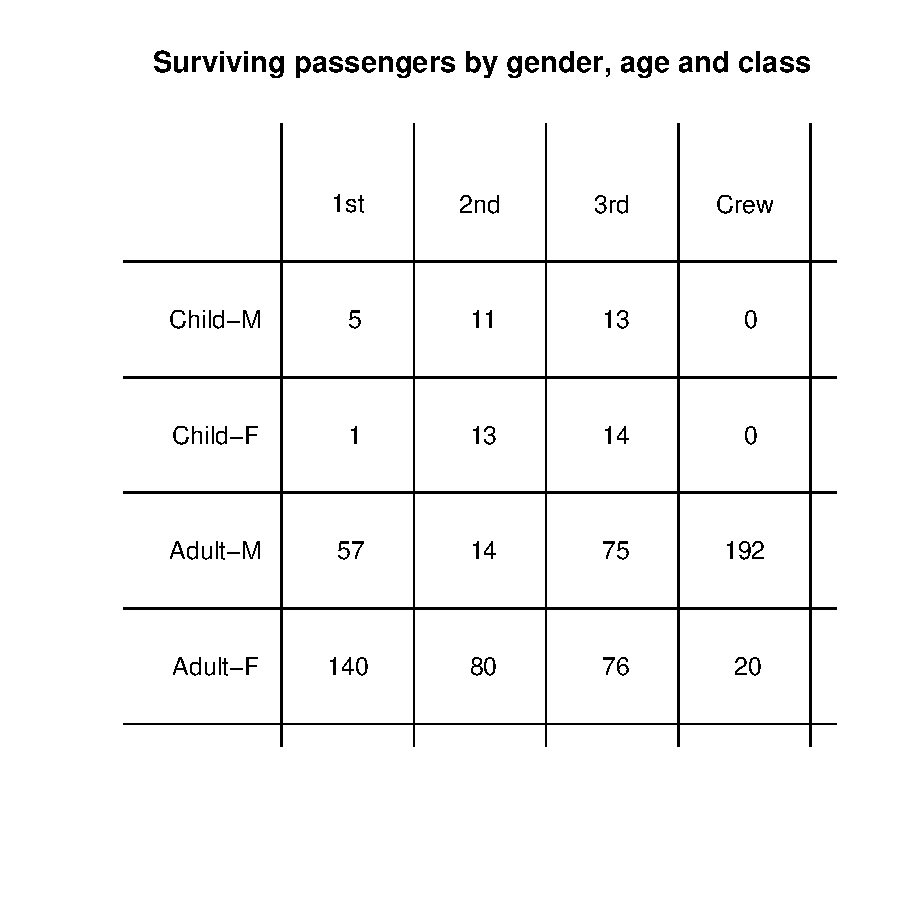
\includegraphics[width=\textwidth]{SurvivedPopWhite.pdf}
\vspace{-0.65in}
\caption{\label{figure:Surv.Pop.White}
Tabular representation of surviving population}
\end{figure}

Figure~\ref{figure:Surv.Pop.White} displays a graphical table
without balloons.  (This was created by calling balloonplot with the
balloon color set to match the background color.)  Note that one
must actively focus on the individual cell values in order to see
any pattern in the data.

Now we redraw this same figure using light blue circles
(Figure~\ref{figure:Surv.Pop}).  This is accomplished using the code:

{\small
\begin{verbatim}
library(gplots)
data(Titanic)

surv.pop <- cbind(Titanic[,,Age="Child", 
                         survived="Yes"],
                  Titanic[,,Age="Adult", 
                         survived="Yes"])
colnames(surv.pop) <- c("Child-M", "Child-F",
                         "Adult-M", "Adult-F")
balloonplot(as.table(surv.pop), xlab="", 
            ylab="", main="")
title("BalloonPlot : Surviving passengers by
 gender and age")
mtext("(Area proportional to frequency)")
\end{verbatim}
 }

\begin{figure}[h]
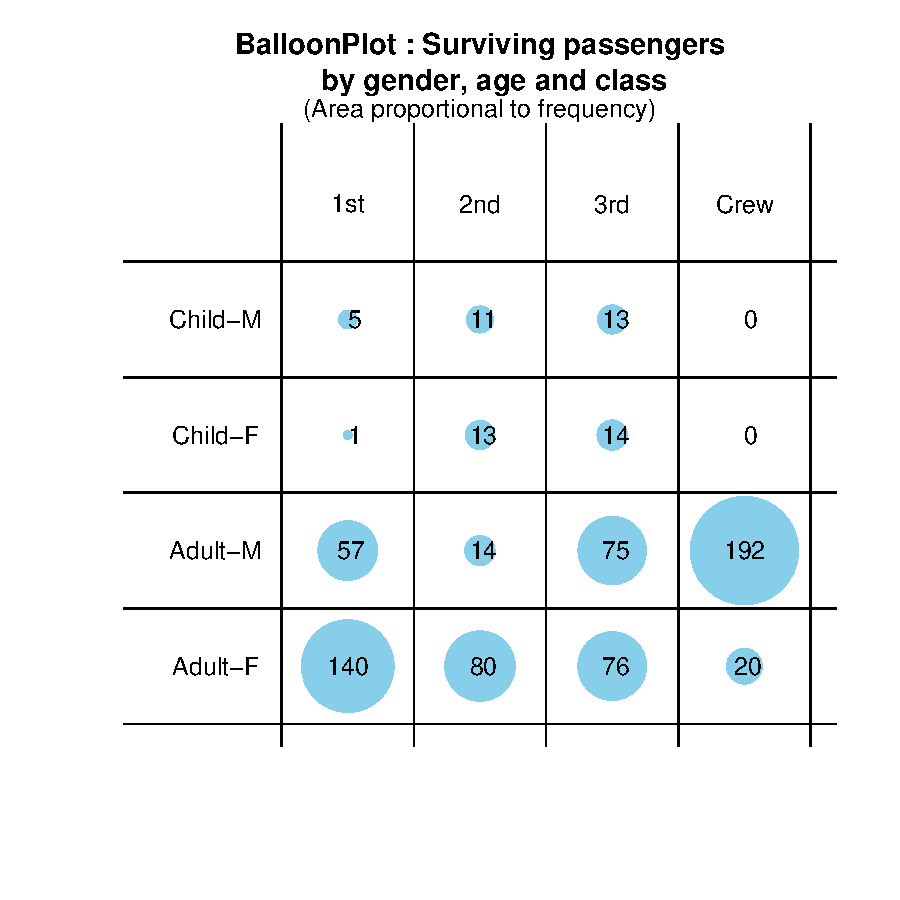
\includegraphics[width=\textwidth]{SurvivedPop.pdf}
\vspace{-0.65in}
\caption{\label{figure:Surv.Pop}
Balloon plot of survived population}
\end{figure}

With the addition of the blue ``spotlights'', it is easy to see that
only adult females and adult male crew members survived in large
numbers.

Let us investigate further, by examining the number
of individuals belonging to each category:

{\small
\begin{verbatim}
total.pop <- cbind(apply(Titanic[,,Age="Child",],
                         c(1,2), sum), 
                   apply(Titanic[,,Age="Adult",], 
                         c(1,2), sum))
colnames(total.pop) <- c("Child-M", "Child-F", 
                         "Adult-M", "Adult-F")
balloonplot(as.table(total.pop), xlab="",
            ylab="", main="")
title("BalloonPlot : Total passengers by
 gender and age")
mtext("(Area proportional to frequency)")
\end{verbatim}
 }

\begin{figure}[h]
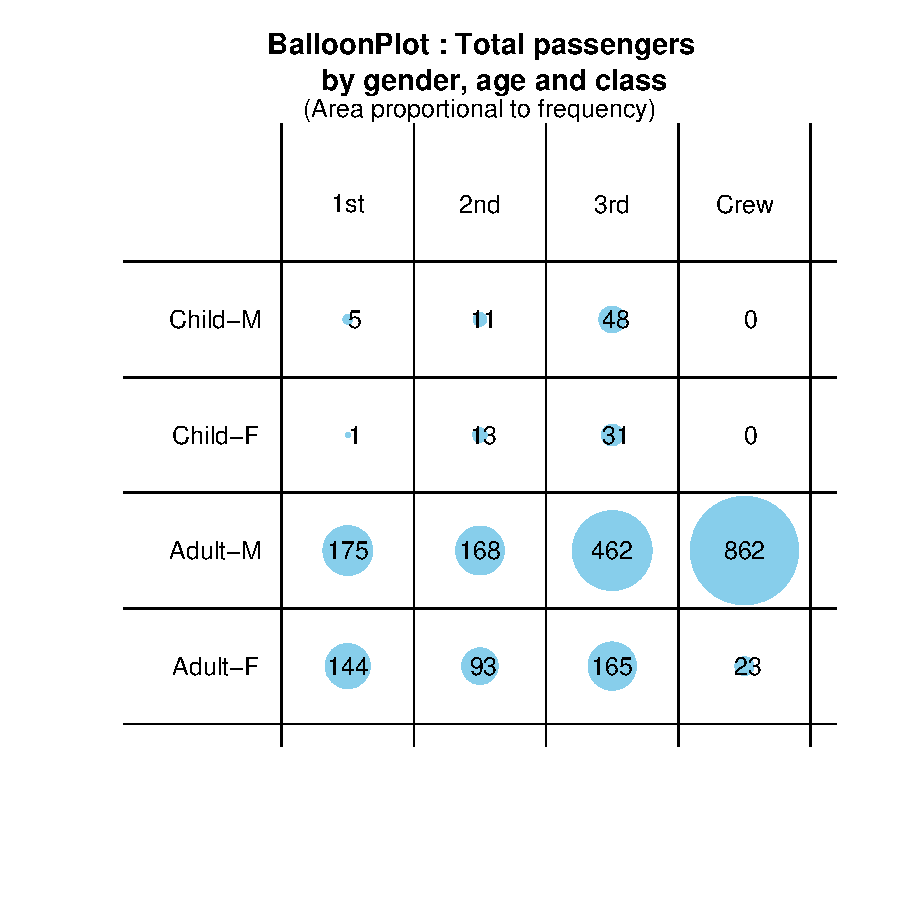
\includegraphics[width=\textwidth]{TotalPop.pdf}
\vspace{-0.65in}
\caption{\label{figure:Total.Pop}
Balloon plot of total population}
\end{figure}

\noindent 
Figure\ref{figure:Total.Pop} shows that the largest number of
individuals on board were adult male crew (862), followed by adult males in
$3^{rd}$ class (462).  Thus it is not surprising that a large number
of adult male crew members survived.  However, we now realize that
survival among $3^{rd}$ class adult males should have been high too.
So, let us look at the fraction of passengers from each group who
survived.

{\small
\begin{verbatim}

surv.prop <- as.table(surv.pop/total.pop)

surv.prop[is.na(surv.prop)] <- 0

balloonplot(as.table(surv.prop), xlab="",
            ylab="", main="")
title("BalloonPlot : Surviving passengers
 by gender and age")
mtext("(Area proportional to frequency)")
\end{verbatim}
}


\begin{figure}[h]
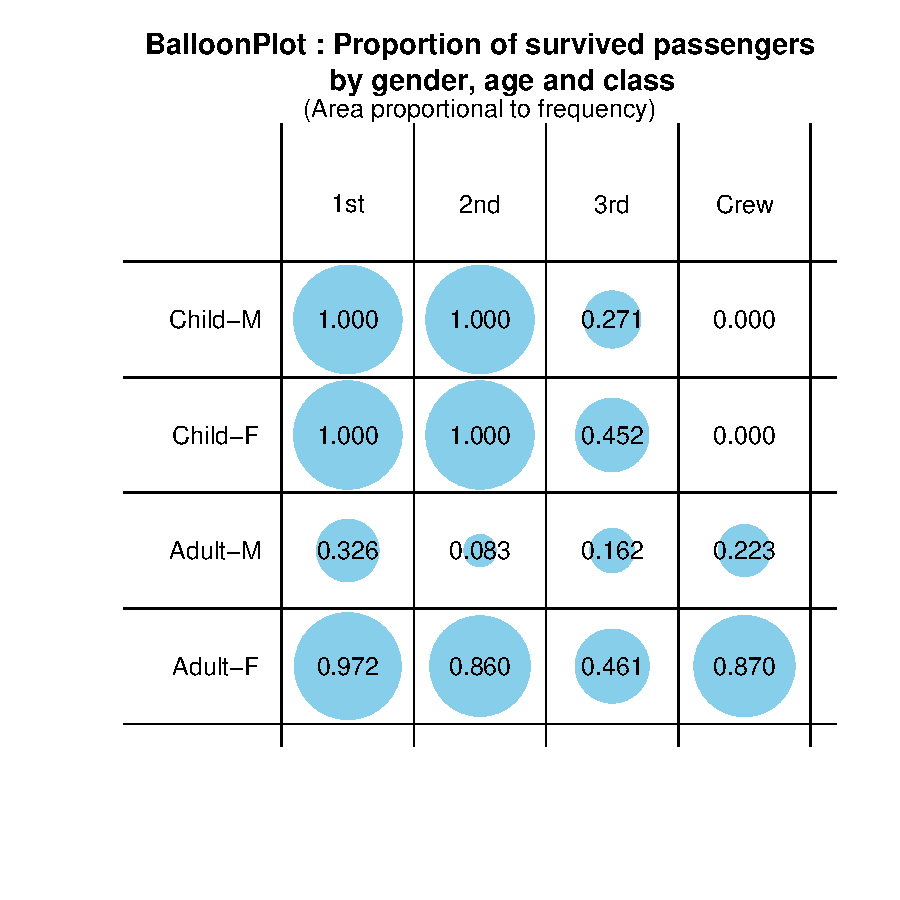
\includegraphics[width=\textwidth]{SurvivedProp.pdf}
\vspace{-0.65in}
\caption{\label{figure:Surv.Prop}
Balloon plot of proportion of people surviving}
\end{figure}

From Figure \ref{figure:Surv.Prop} we can easily see that all the
children in $1^{st}$ and $2^{nd}$ class survived, as did most of the
women in $1^{st}$ and $2^{nd}$ class and among the crew.  It is also
evident that survival among $3^{rd}$ class passengers is much lower
than in any of the other classes.

The reasons for this are well known: 
\begin{enumerate}
  \item Third class passengers were berthed below decks and hence
  had diffuclty reaching the life boat launches.
  \item Once at the lifeboats, women and children had priority.
  \item Titanic had too few lifeboats for the number of passengers and crew.
\end{enumerate}
Thus, most women and children among first and second class
passengers and crew found space in a lifeboat, while most of the
third class passengers never made it to lifeboats, since the
lifeboats had already been filled and had moved away from the
quickly sinking ship.

\section*{Conclusion}

Using the well worn Titanic data, we have shown how balloonplots
help to convey important aspects of tabular data, without obscuring
the exact numeric values. We hope that this new approach to
visualizing tabular data will assist other statiticians in more
effectively understanding and presenting tabular data.

We wish to thank \emph{Ramon Alonso-Allende}
\email{allende@cnb.uam.es} for the discussion on R-help which lead
to the development of \code{balloonplot}.

\address{Gregory R. Warnes, Pfizer Inc., USA\\
\email{gregory.r.warnes@pfizer.com}\\
       Nitin Jain, Pfizer Inc., USA\\
\email{nitin.jain@pfizer.com}}

\begin{thebibliography}{99}
\expandafter\ifx\csname natexlab\endcsname\relax\def\natexlab#1{#1}\fi
\expandafter\ifx\csname url\endcsname\relax
  \def\url#1{{\tt #1}}\fi


\bibitem{Friendly}M. Friendly. 
Mosaic displays for multi-way contingency tables.
\newblock{\em Journal of the
American Statistical Association}, 89:190-200, 1994.

\bibitem{Hartigan}J.\ Hartigan and B.\ Kleiner. 
\newblock Mosaics for contingency tables.
In W. F. Eddy (Ed.), 
\newblock{ \em Computer Science and
Statistics: Proceedings of the 13th Symposium on the Interface.}
268-273, 1981. New
York: Springer-Verlag. 


\end{thebibliography}


\end{article}

\end{document}
